\medskip
\textbf{Partie A}
\medskip
\begin{enumerate}
	\item Puisque l'individu est choisi dans la population française, on suppose qu'il y a une situation d'équiprobabilité et que les proportions sont assimilables à des probabilités.

Comme 5,7\,\% des adultes avaient déjà été infectés, d'après l'étude du \emph{Lancet}, la probabilité que l'individu choisi ait déjà été infecté est de $P(I) = 0,057$.

	\item \begin{enumerate}
		\item \begin{itemize}
			\item On a une épreuve de Bernoulli, dont le succès : \og l'individu choisi a déjà été infecté\fg{}, a une probabilité $p = 0,057$;
			\item Cette épreuve est répétée $N = 100$ fois, de façon identique et indépendante (car le prélèvement des 100 individus est assimilé à un tirage avec remise);
			\item $X$ est une variable aléatoire qui compte le nombre de succès parmi ces répétitions.
		\end{itemize}

		Avec ces éléments, on peut affirmer que $X$ suit la loi binomiale de paramètres $N = 100$ et $p = 0,057$.

		\emph{Remarque :} le paramètre donnant le nombre de répétitions est souvent noté $n$, plutôt que $N$, mais dans la question \textbf{2. e.}, un entier $n$ est introduit, donc pour éviter le conflit de notation, on utilise $N$ ici.

		\item Puisque $X$ suit une loi binomiale, on a :\quad $E(X) = N\times p = 100\times 0,057 = 5,7$. On en déduit que dans un échantillon de 100 personnes adultes choisies au sein de la population française le  11 mai 2020, en moyenne, 5,7 d'entre eux avaient déjà été infectés par la COVID 19.

		\item La probabilité demandée est celle de l'évènement $\{X = 0\}$.

Pour les variables aléatoires régies par la loi binomiale, on a (pour $k$ entier naturel inférieur à $n$) :\quad $P(X = k) = \displaystyle \binom{N}{k} \times p^k \times (1 - p)^{N-k}$.

On a donc, ici : \quad $P(X = 0) = \displaystyle \binom{100}{0 }\times 0,057^0 \times 0,943^{100} = 0,943^{100} \approx 0,0028$.

		\item La probabilité qu'au moins deux personnes de l'échantillon aient été préalablement infectées est de :

$P(X \geqslant 2 ) = 1 - P\big(~\overline{X \geqslant 2}~\big) = 1 - P(X \leqslant 1) = 1 - P(X = 0) - P(X = 1)$. (Certains modèles de calculatrices n'ont pas besoin de ce calcul).

À la calculatrice, on obtient : \quad$P(X \geqslant 2) \approx 0,9801$.

		\item Par exploration à la calculatrice, on constate que pour $n \leqslant 8$, on a une probabilité inférieure ou égale à 0,9, avec $P(X \leqslant 8) \approx 0,8829$ et $P(X \leqslant 9) \approx 0,9408$.

L'entier cherché est 9.

Cela signifie que dans un échantillon de cent adultes choisis dans la population française le 11 mai 2020, il y a plus de neuf chances sur dix que le nombre d'entre eux préalablement infectés par la COVID 19 est inférieur ou égal à 9.
	\end{enumerate}
\end{enumerate}

\medskip
\textbf{Partie B}
\medskip

\begin{enumerate}
	\item L'évènement $I$ est l'évènement déjà utilisé dans la \textbf{Partie A}. On avait $P(I) = 0,057$.

	\begin{itemize}
		\item La description de la \textbf{sensibilité} nous fait comprendre qu'il s'agit de la probabilité conditionnelle : \quad $P_I(T) = 0,8$;
		\item celle de la \textbf{spécificité} indique que est :\quad$P_{\overline{I}}\big(~\overline{T}~\big) = 0,99$.
	\end{itemize}

	Avec ces informations, on peut compléter l'arbre probabilisé :

	\hfill~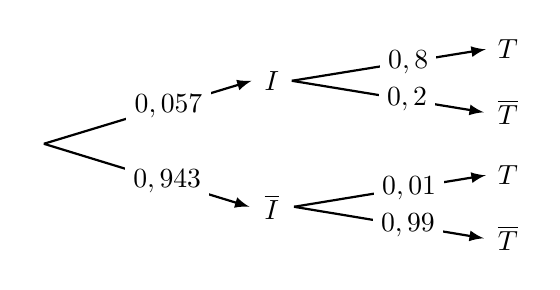
\begin{tikzpicture}[xscale=1,yscale=1,baseline={(R.base)}]
		
		\tikzstyle{fleche}=[->,>=latex,thick]
		\tikzstyle{noeud}=[fill=white,circle,inner sep=2pt]
		\tikzstyle{feuille}=[fill=white,circle,inner sep=2pt]
		\tikzstyle{etiquette}=[pos=0.6,fill=white, inner xsep=3pt, inner ysep=1.5pt]
		
		\def\DistanceInterNiveaux{3}
		\def\DistanceInterFeuilles{0.8}
		
		\def\NiveauA{(0)*\DistanceInterNiveaux}
		\def\NiveauB{(1)*\DistanceInterNiveaux}
		\def\NiveauC{(2)*\DistanceInterNiveaux}
		\def\InterFeuilles{(-1)*\DistanceInterFeuilles}
		
		\node[noeud] (R) at ({\NiveauA},{(1.5)*\InterFeuilles}) {};
		\node[noeud] (Ra) at ({\NiveauB},{(0.5)*\InterFeuilles}) {$I$};
		\node[feuille] (Raa) at ({\NiveauC},{(0)*\InterFeuilles}) {$T$};
		\node[feuille] (Rab) at ({\NiveauC},{(1)*\InterFeuilles}) {$\overline{T}$};
		\node[noeud] (Rb) at ({\NiveauB},{(2.5)*\InterFeuilles}) {$\overline{I}$};
		\node[feuille] (Rba) at ({\NiveauC},{(2)*\InterFeuilles}) {$T$};
		\node[feuille] (Rbb) at ({\NiveauC},{(3)*\InterFeuilles}) {$\overline{T}$};
		
		\draw[fleche] (R.east)--(Ra.west) node[etiquette] {$0,057$};
		\draw[fleche] (Ra.east)--(Raa.west) node[etiquette] {$0,8$};
		\draw[fleche] (Ra.east)--(Rab.west) node[etiquette] {$0,2$};
		\draw[fleche] (R.east)--(Rb.west) node[etiquette] {$0,943$};
		\draw[fleche] (Rb.east)--(Rba.west) node[etiquette] {$0,01$};
		\draw[fleche] (Rb.east)--(Rbb.west) node[etiquette] {$0,99$};
	\end{tikzpicture}\hfill~

	\item Les évènements $I$ et $\overline{I}$ partitionnent l'univers, donc, d'après la loi des probabilités totales :

	$P(T) = P\big(I\cap T\big) + P\big(~\overline{I} \cap T\big) = 0,057 \times 0,8 + 0,943 \times 0,01 = \np{0,05503}$.

	\item La question posée est de calculer : \quad $P_T(I)$.

	D'après la définition des probabilités conditionnelles :

	$P_T(I) = \dfrac{P(T \cap I)}{P(T)} = \dfrac{0,057 \times 0,8}{\np{0,05503}} = \dfrac{4560}{5503} \approx \np{0,8286}$.

	Cela signifie qu'une personne dont le test est positif n'a qu'une probabilité de \np{0,8286} (environ) d'avoir été préalablement infectée par la COVID 19.
	\end{enumerate}

\medskip
\textbf{Partie C}
\medskip

Si le test est le même, sa sensibilité et sa spécificité sont les mêmes, ce qui change, c'est donc la probabilité d'avoir été préalablement infecté. Cette probabilité n'est pas connue, notons la $x$.

On a donc l'arbre suivant :

\hfill~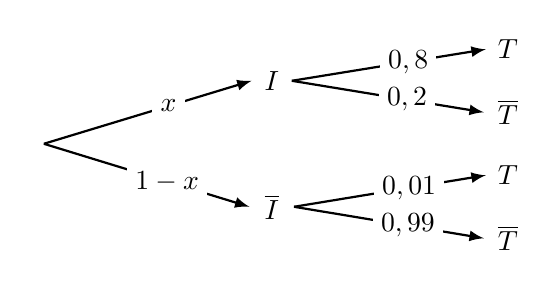
\begin{tikzpicture}[xscale=1,yscale=1,baseline={(R.base)}]
	
	\tikzstyle{fleche}=[->,>=latex,thick]
	\tikzstyle{noeud}=[fill=white,circle,inner sep=2pt]
	\tikzstyle{feuille}=[fill=white,circle,inner sep=2pt]
	\tikzstyle{etiquette}=[pos=0.6,fill=white, inner xsep=3pt, inner ysep=1.5pt]
	
	\def\DistanceInterNiveaux{3}
	\def\DistanceInterFeuilles{0.8}
	
	\def\NiveauA{(0)*\DistanceInterNiveaux}
	\def\NiveauB{(1)*\DistanceInterNiveaux}
	\def\NiveauC{(2)*\DistanceInterNiveaux}
	\def\InterFeuilles{(-1)*\DistanceInterFeuilles}
	
	\node[noeud] (R) at ({\NiveauA},{(1.5)*\InterFeuilles}) {};
	\node[noeud] (Ra) at ({\NiveauB},{(0.5)*\InterFeuilles}) {$I$};
	\node[feuille] (Raa) at ({\NiveauC},{(0)*\InterFeuilles}) {$T$};
	\node[feuille] (Rab) at ({\NiveauC},{(1)*\InterFeuilles}) {$\overline{T}$};
	\node[noeud] (Rb) at ({\NiveauB},{(2.5)*\InterFeuilles}) {$\overline{I}$};
	\node[feuille] (Rba) at ({\NiveauC},{(2)*\InterFeuilles}) {$T$};
	\node[feuille] (Rbb) at ({\NiveauC},{(3)*\InterFeuilles}) {$\overline{T}$};
	
	\draw[fleche] (R.east)--(Ra.west) node[etiquette] {$x$};
	\draw[fleche] (Ra.east)--(Raa.west) node[etiquette] {$0,8$};
	\draw[fleche] (Ra.east)--(Rab.west) node[etiquette] {$0,2$};
	\draw[fleche] (R.east)--(Rb.west) node[etiquette] {$1-x$};
	\draw[fleche] (Rb.east)--(Rba.west) node[etiquette] {$0,01$};
	\draw[fleche] (Rb.east)--(Rbb.west) node[etiquette] {$0,99$};
\end{tikzpicture}\hfill~

	Les évènements $I$ et $\overline{I}$ partitionnent toujours cet univers différent, donc, d'après la loi des probabilités totales :

$P(T) = P\big(I\cap T\big) + P\big(~\overline{I} \cap T\big) = x \times 0,8 + (1 - x) \times 0,01 = 0,8x + 0,01 - 0,01x = 0,79x + 0,01$.

D'après l'énoncé, 29,44\,\% des gens ont un test positif, donc la probabilité de choisir un individu dont le test est positif est de 0,2944.

On a donc une double égalité, dont on déduit l'équation suivante : \quad $0,79x + 0,01 = 0,2944$

Résolvons :\quad $\begin{aligned}[t] 0,79x + 0,01 = \np{0,2944}&\iff 0,79x = \np{0,2844}\\
&\iff x = \dfrac{\np{0,2844}}{0,79}\\
&\iff x = \dfrac{\np{2844}}{\np{7900}}\end{aligned}$

La probabilité que la personne choisie ait été infectée est donc de $\dfrac{\np{2844}}{\np{7900}} = 0,36$.

Dans cet autre pays, la proportion de personnes préalablement infectées est donc 36\,\%.

\bigskip
